\documentclass{article}
\usepackage{amsmath,amsfonts,amsthm,amssymb,amsopn,bm}
\usepackage[margin=.9in]{geometry}
\usepackage{graphicx}
\usepackage{url}
\usepackage[usenames,dvipsnames]{color}
\usepackage{fancyhdr}
\usepackage{multirow}
\usepackage{listings}
\usepackage{hyperref}

\definecolor{keywords}{RGB}{255,0,90}
\definecolor{comments}{RGB}{0,0,113}
\definecolor{red}{RGB}{160,0,0}
\definecolor{green}{RGB}{0,150,0}
 
\lstset{language=Python, 
        basicstyle=\ttfamily\tiny, 
        keywordstyle=\color{keywords},
        commentstyle=\color{comments},
        stringstyle=\color{red},
        showstringspaces=false}

\newcommand{\field}[1]{\mathbb{#1}}
\newcommand{\1}{\mathbf{1}}
\newcommand{\E}{\mathbb{E}} 
\newcommand{\Z}{\mathbb{Z}} 
\renewcommand{\P}{\mathbb{P}}
\newcommand{\R}{\field{R}} % real domain
% \newcommand{\C}{\field{C}} % complex domain
\newcommand{\F}{\field{F}} % functional domain
\newcommand{\T}{^{\textrm T}} % transpose
\def\diag{\text{diag}}

%% operator in linear algebra, functional analysis
\newcommand{\inner}[2]{#1\cdot #2}
\newcommand{\norm}[1]{\left\|#1\right\|}
\newcommand{\twonorm}[1]{\|#1\|_2^2}
% operator in functios, maps such as M: domain1 --> domain 2
\newcommand{\Map}[1]{\mathcal{#1}}
\renewcommand{\theenumi}{\alph{enumi}} 

\newcommand{\Perp}{\perp \! \! \! \perp}

\newcommand\independent{\protect\mathpalette{\protect\independenT}{\perp}}
\def\independenT#1#2{\mathrel{\rlap{$#1#2$}\mkern2mu{#1#2}}}
\newcommand{\vct}[1]{\boldsymbol{#1}} % vector
\newcommand{\mat}[1]{\boldsymbol{#1}} % matrix
\newcommand{\cst}[1]{\mathsf{#1}} % constant
\newcommand{\ProbOpr}[1]{\mathbb{#1}}
\newcommand{\points}[1]{\small\textcolor{magenta}{\emph{[#1 points]}} \normalsize}
\date{{}}

\setlength\parindent{0px}

\begin{document}
\title{Homework \#2}
\author{\normalsize{Winter 2020, STATS 509}\\
\normalsize{Dino Bektesevic}}
\maketitle

\section*{Problem 1}
\begin{enumerate}
	\item in this case k=1 so the winnings can only be 0 or 2/3, i.e. $X_1=\{0, 2/3\}$. The probability of each coin toss is 1/2. We can write the pmf function as:
	$$f(x) = \begin{cases} 
	        1/2 &\mbox{if } x \in X_1 \\
            0 & \mbox{if } x \notin X_1 
        \end{cases} 
    $$
    essentially saying that the probability of seeing random variable $x$ be either win or lose is 50 percent. the cumulative distribution function, i.e. cdf, is given by $F_X(x) = P(X\leq x) = \sum_i p(x_i)$. In our case this boils down to three cases, corresponding to the two mass points - a win or no win:
	$$F(x) = \begin{cases} 
	        0 &\mbox{if } x < 0 \\
	        1/2 &\mbox{if } 0 \leq x \leq 2/3 \\
            1 & \mbox{if } x > 2/3 
        \end{cases} 
    $$

    \item in case of k=2 there are 4 different winnings $X_2=\{0, 2/3, 2/9, 8/9\}$ corresponding to four outcome cases (where ordering matters) $x=\{tt, ht, th, hh\} = \{\mbox{0+0}, \mbox{2/3+0}, \mbox{0+2/9}, \mbox{2/3+2/9}\}$. The probability of each outcome is 1/4 because these are two independent events each with probability of 1/2. Written down:
    $$f(x) = \begin{cases} 
	        1/4 &\mbox{if } x \in X_2 \\
            0 & \mbox{if } x \notin X_2 
        \end{cases} 
    $$
	Similarly there are now 5 cases corresponding to the 4 mass points in the cdf:
	$$F(x) = \begin{cases} 
	        0 &\mbox{if } x < 0 \\
	        0.25 &\mbox{if } 0\leq x \leq 2/9 \\
            0.5  & \mbox{if } 2/9 < x \leq 2/3 \\
            0.75 & \mbox{if } 2/3 < x \leq 8/9 \\
            1 & \mbox{if } x > 8/9
        \end{cases} 
    $$
	
	\newpage
	\item I run a million simulations counting up all the winnings from each toss in each simulation in Python.
	\begin{center}
    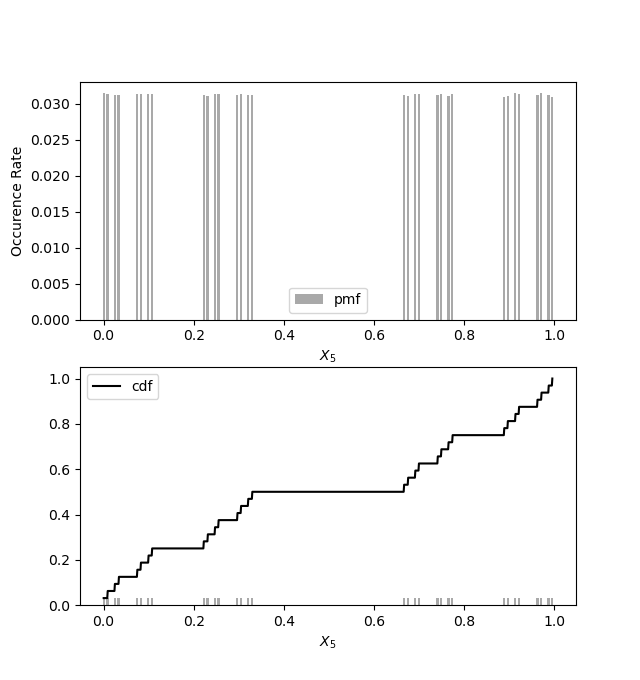
\includegraphics[width=2.5in]{STATS509/HW2/HW2Figures/problem1c.png}
    \end{center}
    \lstinputlisting[language=Python]{HW2Code/HW2_Problem1.py}
\end{enumerate}


\newpage
\section*{Problem 2}
\begin{center}
    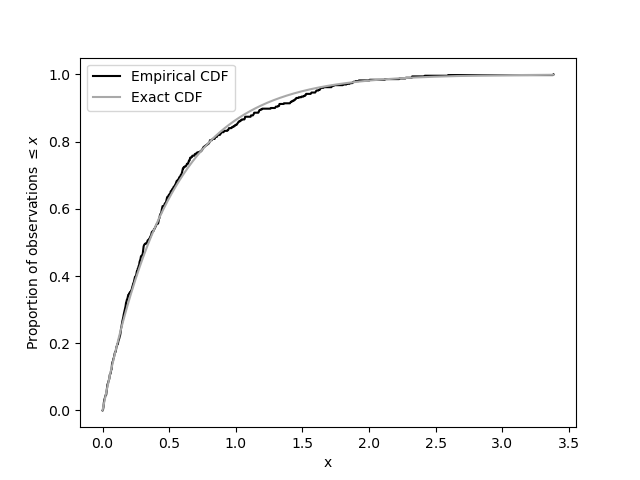
\includegraphics[width=3in]{STATS509/HW2/HW2Figures/problem2.png}
\end{center}
\lstinputlisting[language=Python]{HW2Code/problem2.py}


\newpage
\section*{Problem 3}
\begin{enumerate}
	\item As in all the problems above the empirical CDF is just a counting function:
	$$\F(t) = \frac{1}{n}\sum_{i=1}^n \1\{x_i\leq t\}$$
	
	\item I assume Rectangular distribution is the Uniform distribution given by:
	$$ f(x)=\begin{cases}
            \frac{1}{b - a} & \mathrm{for}\ a \le x \le b, \\
            0 & \mathrm{for}\ x<a\ \mathrm{or}\ x>b
            \end{cases}
    $$
    In this problem we are given that $b=1$ and $a=0$ so that $f(t)=1$ for $0\leq t \leq 1$. CDF, given by the definition $\F(x) = \int f(x) dx$, in this problem is then:
    $$ \F(t) = \int_{-\infty}^{\infty} f(t) dt = 
        \begin{cases}
            0 & \mathrm{for}\ t < 0 \\
            \int_0^tdt = t & \mathrm{for}\ 0 \leq t \leq 1 \\
            1 & \mathrm{for}\  t > 1
        \end{cases}
    $$
    
    \item 
    
    
\end{enumerate}	
	
	
\newpage
\section*{Problem 4}


\newpage
\section*{Problem 5}


\newpage
\section*{Problem 6}


\newpage
\section*{Problem 7}


\end{document}
